\documentclass[12pt,a4paper]{article}
\usepackage[utf8]{inputenc}
\usepackage[OT1]{fontenc}
\usepackage{amsmath}
\usepackage{amsfonts}
\usepackage{amssymb}
\usepackage{graphicx}
\usepackage{tikz}
\usepackage{pgfplotstable}
\usepackage{mathtext}

\usepackage[T1]{fontenc}
\usepackage[utf8]{inputenc}
\usepackage[english, bulgarian, russian]{babel}

\usepackage{tikz}
\usepackage{pgfplots}
\usepackage{indentfirst}
\usepackage[export]{adjustbox}
\usepackage{multirow}
\usepackage{geometry} \geometry{verbose,a4paper,tmargin=2cm,bmargin=2cm,lmargin=1.5cm,rmargin=1.5cm}

\graphicspath{{Images/}}
\usepackage[left=2cm,right=2cm,top=2cm,bottom=2cm]{geometry}
\usepackage{wrapfig}
\usepackage{setspace}
\usepackage{indentfirst}
\usepackage{subfigure}


\begin{document}

\begin{titlepage}
  \begin{center}
    \huge
    Московский Физико-технический Институт
    
    (Национальный исследовательский университет)
    \vspace{0.5cm}

   
    \vspace{0.25cm}
 
    \vfill
 
    \vfill

    \textsc{\bf{Отчет о выполнении работы 2.1.3}}\\[3mm]
    
    {\LARGE  Определение $C_p/C_v$ по скорости звука в газе}
  \bigskip
    \vfill
    
\end{center}
\vfill
\begin{flushright}

    Выполнили студентки 1 курса
    
    ФБМФ, группа Б06-103

    Попеску Полина
    
    
    Фитэль Алёна

\end{flushright}
\bigskip


\vfill

\begin{center}
  Долгопрудный, 2022 г.
\end{center}
\end{titlepage}

\section{Введение}

\textbf{Цель работы:} 1) измерение частоты колебаний и длины волны при резонансе звуковых колебаний в газе; 2) определение показателя адиабаты с помощью уравнения состояния идеального газа.

\textbf{В работе используются:} звуковой генератор ГЗ; электорнный осциллограф ЭО; микрофон; телефон; раздвижная труба; теплоизолированная труба, обогреваемая водой из термостата; баллон со сжатым углекислым газом; газгольдер.

\section{Теоретические сведения}

Скорость распространения звуковой волны в газах зависит от показателя адиабаты $ \gamma $. На измерении скорости звука основан один из наиболее точных методов определения показателя адиабаты.

Скорость звука в газах определяется формулой:

\begin{equation}\label{velocity}
c=\sqrt{\gamma\frac{RT}{\mu}}.
\end{equation}
где $ R $ -- газовая постоянная, $ T $ -- температура газа, а $ \mu $ -- его молярная масса. Преобразуя эту формулу, найдем
\begin{equation}\label{gamma}
\boxed{\gamma = \frac{\mu}{RT}c^2}.
\end{equation}

Таким образом, для определения показателя адиабаты достаточно измерить температуру газа и скорость распространения звука (молярная масса газа предполагается известной).

Звуковая волна, распространяющаяся вдоль трубы, испытывает многократные отражения от торцов. Звуковые колебания в трубе являются наложением всех отраженных волн и очень сложны. Картина упрощается, если длина трубы $ L $ равна целому числу полуволн, то есть когда \[ L=n\lambda/2, \] где $ \lambda $ -- длина волны звука в трубе, а $ n $ -- любое целое число. Если это условие выполнено, то волна, отраженная от торца трубы, вернувшаяся к ее началу и вновь отраженная, совпадает по фазе с падающей. Совпадающие по фазе волны усиливают друг друга. Амплитуда звуковых колебаний при этом резко возрастает -- наступает резонанс.

При звуковых колебаниях слои газа, прилегающие к торцам трубы, не испытывают смещения. Узлы смещения повторяются по всей длине трубы через $ \lambda/2 $. Между узлами находятся максимумы смещения.

Скорость звука c связана с его частотой $ f $ и длиной волны $ \lambda $ соотношением

\begin{equation}\label{lambda_f}
c=\lambda f.
\end{equation}

Подбор условий, при которых возникает резонанс, можно производить двояко:
\begin{enumerate}
	\item При постоянной длине трубы можно изменять частоту звуковых колебаний. В этом случае следует плавно изменять частоту $ f $ звукового генератора, а следовательно, и длину звуковой волны $ \lambda $. Для последовательных резонансов получим 
	\begin{equation}\label{4}
	L=\frac{\lambda_1}{2}n=\frac{\lambda_2}{2}(n+1)=\dots=\frac{\lambda_{k+1}}{2}(n+k).
	\end{equation}
	
	Из \eqref{lambda_f} и \eqref{4} имеем:
	\[ f_1=\frac{c}{\lambda_1}=\frac{c}{2L}n, \quad f_2=\frac{c}{\lambda_2}=\frac{c}{2L}(n+1)=f_1+\frac{c}{2L},\quad \dots, \]
	\begin{equation}\label{5}
	f_{k+1}=\frac{c}{\lambda_{k+1}}=\frac{c}{2L}(n+k)=f_1+\frac{c}{2L}k.
	\end{equation}
	Скорость звука, деленная на $ 2L $, определяется, таким образом, по угловому коэффициенту графика зависимости частоты от номера резонанса.
	\item При неизменной частоте $ f $ звукового генератора (а следовательно, и неизменной длине звуковой волны $ \lambda $) можно изменять длину трубы $ L $. Для этого применяется раздвижная труба. Длина раздвижной трубы постепенно увеличивается, и наблюдается ряд последовательных резонансов. Возникновение резонанса легко наблюдать на осциллографе по резкому увеличению амплитуды колебаний. Для последовательных резонансов имеем \begin{equation}\label{first}
	L_n=n\frac{\lambda}{2}, \quad L_{n+1}=(n+1)\frac{\lambda}{2}, \quad \dots, \quad L_{n+k} = n\frac{\lambda}{2}+k\frac{\lambda}{2},
	\end{equation} т. е. $ \lambda/2 $ равно угловому коэффициенту графика, изображающего зависимость длины трубы $ L $ от номера резонанса $ k $. Скорость звука находится по формуле \eqref{lambda_f}.
\end{enumerate}

 
\section{Обработка результатов измерений}
\subsection{Измерение $ C_p/C_v $ для воздуха при различных температурах}

Проведём измерения $ C_p/C_v $ для воздуха при различных температурах. Для этого будем использовать трубу постоянного размера $ L = (740 \pm 1) $ мм. Для фиксированной температуры будем изменять частоту звукового сигнала, тем самым изменяя и длину волны, так, чтобы мы могли наблюдать последовательные резонансы. Для каждого резонанса будем фиксировать частоту, при которой он возник. Полученные измерения и величину $ f_k = \hat{f_k} - \hat{f_0} $ занесём в таблицу \ref{tab:constL}.

\begin{table}[!h]
	\centering
	\begin{tabular}{|c|c|c|c|c|c|c|c|c|c|c|}
		\hline
		$ T $, К & \multicolumn{2}{c|}{296,4} & \multicolumn{2}{c|}{303,1} & \multicolumn{2}{c|}{309,6} & \multicolumn{2}{c|}{316,3} & \multicolumn{2}{c|}{322,3} \\ \hline
		k & $ \hat{f_k} $, Гц & $ f_k $, Гц & $ \hat{f_k} $, Гц & $ f_k $, Гц & $ \hat{f_k} $, Гц & $ f_k $, Гц & $ \hat{f_k} $, Гц & $ f_k $, Гц & $ \hat{f_k} $, Гц & $ f_k $, Гц \\ \hline
	    2 & 477 &  0  & 482 & 0 & 486 & 0 & 495 & 0 & 497 & 0 \\ \hline
		3 & 704 & 227 & 712 & 230 & 719 & 233 & 727 & 232 & 733 & 236\\ \hline
		4 & 933 & 456 & 943 & 461 & 953 & 467 & 962 & 467 & 972 & 475 \\ \hline
		5 & 1162 & 685 & 1175 & 693 & 1187 & 701 & 1200 & 705 & 1211 & 714 \\ \hline
		6 & 1394 & 917 & 1409 & 927 & 1423 & 937 & 11438 & 943 & 1452 & 955 \\ \hline
		7 & - & - & 1641 & 1159 & 1658 & 1172 & 1676 & 1181 & 1692 & 1195 \\ \hline
	\end{tabular}
	\caption{Результаты измерений при разных температурах для воздуха}
	\label{tab:constL}
\end{table}
По полученным экспериментальным данным построим графики зависимости $ f_k(k) $.
Аппроксимируем полученные зависимости прямыми $ y=ax $ используя метод наименьших квадратов. Результаты вычислений для каждой температуры заносим в таблицу \ref{tab:resConstL}. Согласно формуле \eqref{5}, коэффициент наклона $ \displaystyle a = \frac{c}{2L}$. Тогда вычислим скорость звука $ c $ при фиксированной температуре и её погрешность, по формуле \eqref{gamma} вычислим $ \gamma $ при фиксированной температуре и погрешность этого вычисления. Результаты также занесём в таблицу $ \ref{tab:resConstL} $.
\newpage
 \begin{figure}[h!]
    \centering
    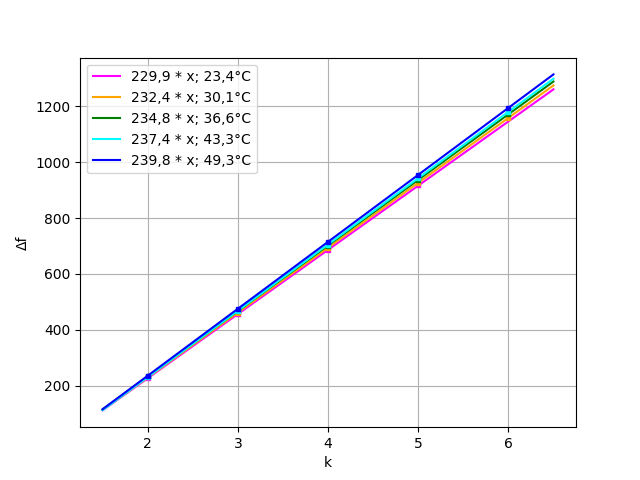
\includegraphics[scale=0.75]{plot.png}
    \caption {График зависимости $ f_k(k) $}
\end{figure}
\begin{table}[h!]
	\centering
	\begin{tabular}{|c|c|c|c|c|c|c|}
		\hline
		$ T $, К & $ a $, с$ ^{-1} $ & $ \sigma_a $, с$ ^{-1} $ & $ c $, м/с & $ \sigma_c $, м/с & $ \gamma $ & $ \sigma_\gamma $ \\ \hline
		296,4 & 293,4 & 0,3 & 343,6 & 0,6 & 1,362 & 0,005 \\ \hline
		303,1 & 290,9 & 0,3 & 345,6 & 0,6 & 1,361 & 0,005 \\ \hline
		309,6 & 237,2 & 0,3 & 351,1 & 0,6 & 1,360 & 0,005 \\ \hline
		316,3 & 238,9 & 0,3 & 353,6 & 0,6 & 1,361 & 0,005 \\ \hline
		322,3 & 240,1 & 0,3 & 355,4 & 0,6 & 1,363 & 0,005 \\ \hline
	\end{tabular}
	\caption{Результаты вычислений при различных температурах}
	\label{tab:resConstL}
\end{table}
Согласно полученным данным, можно утверждать, что $ \gamma $ остаётся постоянной в исследуемом диапазоне температур. Поэтому усредним результаты, полученные при различных значениях температуры и получим для воздуха:

\[ \boxed{\gamma = 1,361 \pm 0,005}\quad (\varepsilon=0,4\%) \]


\subsection{Измерение $ C_p/C_v $ для углекислого газа при помощи установки с раздвижной трубой}

\label{ident}

Проведём измерение коэффициента $ C_p/C_v $ для углекислого газа при помощи установки с раздвижной трубой. Для проведения серии измерений фиксируем частоту звукового сигнала и оставляем её неизменной до окончания снятия показаний. Увеличиваем длину трубки, чтобы добиться резонанса, возникновение которого устанавливается при помощи осциллографа.
\newpage
При возникновении резонанса фиксируем то расстояние, на которое была выдвинута трубка прибора. Данные измерения проводим для нескольких значений частот.  Также для каждого измерения вычислим $ L_k = l_k - l_0 $. Полученные результаты заносим в таблицу \ref{tab:oxy}.

\begin{table}[!h]
\centering
\begin{tabular}{|c|cc|cc|cc|cc|cc|}
\hline
\multicolumn{1}{|c|}{$f$, Гц} & \multicolumn{2}{c|}{3334}                          & \multicolumn{2}{c|}{1911}                               & \multicolumn{2}{c|}{2496}                               & \multicolumn{2}{c|}{3022}                               & \multicolumn{2}{c|}{3198}                               \\ \hline
$k$                           & \multicolumn{1}{c|}{$l_k$, мм} & $L_k$, мм                 & \multicolumn{1}{c|}{$l_k$, мм} & \multicolumn{1}{c|}{$L_k$, мм} & \multicolumn{1}{c|}{$l_k$, мм} & \multicolumn{1}{c|}{$L_k$, мм} & \multicolumn{1}{c|}{$l_k$, мм} & \multicolumn{1}{c|}{$L_k$, мм} &  \multicolumn{1}{c|}{$l_k$, мм} & \multicolumn{1}{c|}{$L_k$, мм} \\ \hline
 0                          & \multicolumn{1}{c|}{3,8}   & 0                      & \multicolumn{1}{c|}{10,9}  & \multicolumn{1}{c|}{0}     & \multicolumn{1}{c|}{4,6}   &     0                      & \multicolumn{1}{c|}{0,2}   &    0                       & \multicolumn{1}{c|}{4,7}   &               0            \\ \hline
1                           & \multicolumn{1}{c|}{8,3}   & 4,5                   & \multicolumn{1}{c|}{18,8}  & \multicolumn{1}{c|}{7,9}   & \multicolumn{1}{c|}{10,6}  & 6                          & \multicolumn{1}{c|}{5,3}   & 5,1                        & \multicolumn{1}{c|}{9,5}   & 4,8                        \\ \hline
2                           & \multicolumn{1}{c|}{12,7}  & 8,9                   & \multicolumn{1}{c|}{}      &                            & \multicolumn{1}{c|}{16,6}  & 12                         & \multicolumn{1}{c|}{10,3}  & 10,1                       & \multicolumn{1}{c|}{14,4}  & 9,7                        \\ \hline
3                           & \multicolumn{1}{c|}{17}    & 13,2                  & \multicolumn{1}{c|}{}      &                            & \multicolumn{1}{c|}{22,5}  & 17,9                       & \multicolumn{1}{c|}{15,5}  & 15,3                       & \multicolumn{1}{c|}{19,3}  & 14,6                       \\ \hline
4                           & \multicolumn{1}{c|}{}      & \multicolumn{1}{c|}{} & \multicolumn{1}{c|}{}      &                            & \multicolumn{1}{c|}{}      & \multicolumn{1}{c|}{}      & \multicolumn{1}{c|}{20,4}  & 20,2                       & \multicolumn{1}{c|}{}      & \multicolumn{1}{c|}{}      \\ \hline
\end{tabular}	
\caption{Результаты измерений для углекислого газа}
	\label{tab:oxy}
\end{table}



По полученным данным построим графики зависимости $ L_k(k) $.
Аппроксимируем полученные зависимости прямыми $ y=ax $ используя метод наименьших квадратов. Результаты вычислений заносим в таблицу \ref{tab:resO2}. Согласно \eqref{first}, угловой коэффициент наклона прямой $ a $ равен $ \lambda/2 $. Согласно \eqref{lambda_f}, скорость звука в воздухе можно вычислить по следующей формуле: 
\[ c = \lambda f. \]
По формуле \eqref{gamma} вычислим $ C_p/C_v $:

\[ \frac{C_p}{C_v} = \gamma = \frac{\mu}{RT}c^2. \]

При этом для воздуха $ \displaystyle \mu \approx 0,02898 \text{ } \frac{\text{кг}}{\text{моль}} $. Во время эксперимента температура в лаборатории равнялась $ T = (23,4 \pm 0,2) \text{ } ^\circ C $.
Результаты этих вычислений также занесем в таблицу \eqref{lambda_f}. 
 \begin{figure}[h!]
    \centering
    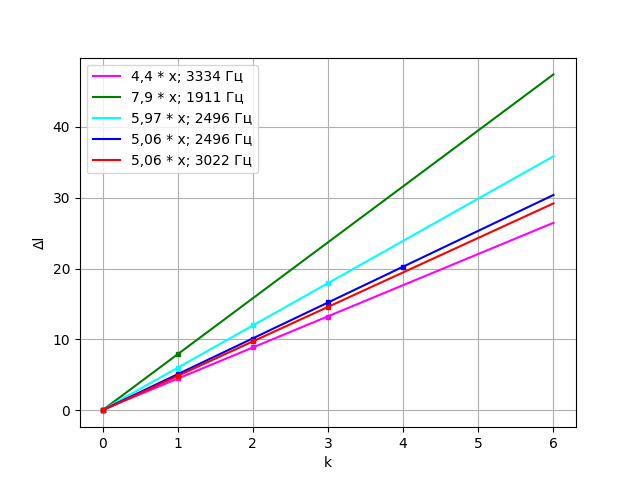
\includegraphics[scale=0.8]{plot2.png}
    \caption {График зависимости $ L_k(k) $}
\end{figure}


\begin{table}[!h]
	\centering
	\begin{tabular}{|c|c|c|c|c|c|c|c|c|}
		\hline
		$ f $, Гц & $ a $, мм & $ \sigma_a $, мм & $ \lambda $, мм & $ \sigma_\lambda $, мм & $ c $, м/с & $ \sigma_c $, м/с& $ \gamma  $ & $ \sigma_\gamma  $ \\ \hline
		3334 & 44,0 & 0,1 & 88,0 & 0,1 & 273 & 2 & 1,338 &0,016\\ \hline
		1911 & 79,0 & 0,2 & 158,0 & 0,2 & 261,94 & 0,16  & 1,429&0,002\\ \hline
		2496 & 59,7 & 0,1 & 119,4 & 0,1 & 268,0 & 0,6 &1,387 & 0,007 \\ \hline
		3022 & 50,6 & 0,1 & 101,2 & 0,1 & 271 & 1  &1,471 &0,012\\ \hline
		3198 & 48,7 & 0,1 & 97,4 & 0,1 & 273,5 & 0,8 & 1,433&0,009\\ \hline
	\end{tabular}
	\caption{Результаты вычислений для углекислого газа}
	\label{tab:resO2}
\end{table}




Таким образом, мы получили значение $ c $ для каждого отдельного значения частоты. Усредняя вычисленные значения, в итоге получаем: \[\boxed{ c = (302,0 \pm 0,5) \text{ м/с}}\quad (\varepsilon=0,17\%) \]
Аналогично было полученно значение $\gamma$ для каждого отдельного значения частоты. Усредняя вычисленные значения, в итоге получаем: 
\[ \boxed{\gamma = 1,411 \pm 0,005}\quad (\varepsilon=0,3\%) \]


\section{Вывод}


В первой части работы был измерен показатель адиабаты для воздуха. Измерения проводились на установке, на которой длина трубы оставалась постоянной на протяжении всего опыта, а резонанс частот получался при помощи изменения частоты звукового сигнала. В ходе этих измерений исследовалась зависимость коэффициента адиабаты $ \gamma $ от температуры газа. Было получено, что показатель адиабаты не зависит от температуры в диапазоне температур $ 20-60 $ $ ^\circ C $ и равняется:

\[ \boxed{\gamma = 1,361 \pm 0,005}\quad (\varepsilon=0,4\%) \]

Сравним полученные данные с табличными. Согласно справочнику, показатель адиабаты для воздуха при стандартных условиях равен \underline{$ \gamma = 1,400 $}. Таким образом, можно утверждать, что результат измерения $ \gamma $ на данной установке несколько отличается от табличного. Это может быть связано с неточностью определения резонансных частот. Чтобы этого избежать, необходимо использовать генератор частоты с возможностью более точной настройки для возможности чёткого отслеживания резонансов.


Во второй части работы был измерен показатель адиабаты для углекислого газа. Измерения проводились при фиксированной частоте звукового сигнала и изменении длины трубы. В итоге было получено значения показателя адиабаты для углекислого газа: \[ \boxed{\gamma = 1,411\pm0,005}\quad (\varepsilon=0,3\%) \] Сравним эти данные с табличными. Согласно справочнику, показатель адиабаты для углекислого газа при стандартных условиях \underline{$ \gamma = 1,300 $}. Полученные данные отличаются от табличных. Это может быть связано с тем, что при измерениях в трубе находился углекислый газ с примесями воздуха, которые могли дать искажения результатов измерений. Для повышения точности, эксперимент стоит проводить в атмосфере углекислого газа, чтобы исключить попадание различных примесей в трубу.











\end{document}
